%!TEX root = ../thesis.tex

\chapter{The title of chapter one}


\section{Quick examples}

Example of citation~\cite{dummy-1} and~\cite{dummy-2}.


Write \(\N,\Z,\Q,\R,\C\).

\(\norm{a}, \abs{b}, \ket{c}, \bra{d}, \braket{e}{f}, \inpro{g}{h}, \nicefrac{3}{\pi}\)

\begin{theorem}
  \label{thm:dummy-thm}
  A
\end{theorem}

\begin{theorem*}[Theorem of second dummy]
  A, follows from Theorem~\ref{thm:dummy-thm}
\end{theorem*}

\begin{lemma}
  \label{lem:dummy}
  Statement
\end{lemma}


\begin{example}
  \label{exa:haha}
  Null example.
\end{example}

\begin{equation}
  \label{eq:nontrivial}
  x^2=x^2.
\end{equation}
Note that Equation~\eqref{eq:nontrivial} is not an obvious fact. You need to scratch your head for it.

\begin{definition}
  \label{def:empty}
  This defintion is not empty.
\end{definition}
\begin{remark}
  \label{rem:regarding-def}
  The reader may find Definition~\ref{def:empty} nonempty, however, you can prove that the definition \emph{is} empty.
\end{remark}

List of environments can be found in the .cls file.



Commutative diagramme using tikz-cd.

\[
  \begin{tikzcd}
  T
\arrow[drr, bend left, "x"]
\arrow[ddr, bend right, "y"]
\arrow[dr, dotted, "{(x,y)}" description] & & \\
& X \times_Z Y \arrow[r, "p"] \arrow[d, "q"] & X \arrow[d, "f"] \\
& Y \arrow[r, "g"] &Z
\end{tikzcd}
\]


Example of commutative diagramme using TikZ.
    \begin{center}
      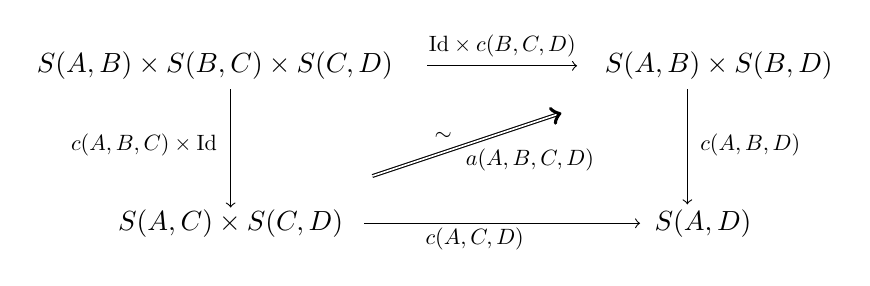
\begin{tikzpicture}[scale=1]
        \draw[->] (1.7,0)--(5.2,0); \draw[->] (0,1.7)--(0,0.2);
        \draw[->](2.5,2)--(4.4,2); \draw[->] (5.8, 1.7)--(5.8,0.24);
        \draw[->, double] (1.8, 0.6)--(4.2,1.4); \node at (6, 0)[
        scale=1]{$\mathfrak{S}(A,D)$}; \node at (6.2, 2)[
        scale=1]{$\mathfrak{S}(A,B)\times \mathfrak{S}(B,D)$}; \node
        at (-0.2, 2)[
        scale=1]{$\mathfrak{S}(A,B)\times \mathfrak{S}(B,C)\times
          \mathfrak{S}(C,D)$}; \node at (2.7,1.1)[scale=0.8]{$\sim$};
        \node at (3.8,0.8)[scale=0.8]{$a(A,B,C,D)$}; \node at (0, 0)[
        scale=1]{$\mathfrak{S}(A,C)\times \mathfrak{S}(C,D)$}; \node
        at (3.45, 2.25)[scale=0.8]{$\textup{Id}\times c(B,C,D)$};
        \node at (-1.1,
        1.0)[scale=0.8]{$ c(A,B,C)\times \textup{Id}$}; \node at (3.1,
        -0.2)[scale=0.8]{$c(A,C,D)$}; \node at (6.6,
        1.0)[scale=0.8]{$c(A,B,D)$};
      \end{tikzpicture}
    \end{center}

    Commutative diagramme using package XY.
    
    \begin{figure}[htb]
      \[
        \xymatrix@1@C=3em{ (G,\alpha)\quad
      \ar@/^1pc/[r]^{(X,\lambda)}_{}="0"
      \ar@/_1pc/[r]_{(Y,\kappa)}^{}="1" \ar@{=>}"0";"1"^{\phi} &
      \quad(H,\beta)\quad \ar@/^1pc/[r]^{(X',\lambda')}_{}="0"
      \ar@/_1pc/[r]_{(Y',\kappa')}^{}="1" \ar@{=>}"0";"1"^{\phi'}&
      \quad(K,\mu) }
  \]
    \caption{}
    \label{fig:vert-comp}
  \end{figure}


  Refer the packages for details about commutative diagrammes (type
  \verb+ texdoc tikz-cd+ or
  \verb+ texdoc xy+ and enter, or ask the internet).


 Glossaries ---regular glossaries, or glossaries appearing as list of
 symbols, etc--- are supported with package \emph{glossaries}. It can
 be used in the standard way. The package does not have \emph{xindy} option.

 Package \emph{xcolor} is loaded with \emph{x11names} option.

 Avoid working out~\ref{rem:more-details} and~\ref{rem:renaming-env}
 unless you know what you are doing.
 \begin{remark}
   \label{rem:more-details}
   Please have a look at \emph{commands.tex} and \emph{symbols.tex},
   in commands folder, for various shortforms and newcommands. You may
   modify and add new newcommands here. The packages are listed in
   IISERB.cls. You may add or modify the packages as per your need.
 \end{remark}
  
  \begin{remark}
    \label{rem:renaming-env}
    If you want, you may modify the math-theorem commands to use
    \verb+ \begin{thm}+ instead of
    \verb+ \begin{theorem}+ , and similar
    for other environments like proposition, examples, remarks. Check
    out the \emph{command.tex} in the commands folder.
  \end{remark}
  
\section{Dummy text}

In mathematics, a group is a set equipped with a binary operation that combines any two elements to form a third element in such a way that four conditions called group axioms are satisfied, namely closure, associativity, identity and invertibility. One of the most familiar examples of a group is the set of integers together with the addition operation, but groups are encountered in numerous areas within and outside mathematics, and help focusing on essential structural aspects, by detaching them from the concrete nature of the subject of the study.

\section{Philosophical discussion about groups}
\label{sec:grp-philo}

Groups share a fundamental kinship with the notion of symmetry. For example, a symmetry group encodes symmetry features of a geometrical object: the group consists of the set of transformations that leave the object unchanged and the operation of combining two such transformations by performing one after the other. Lie groups are the symmetry groups used in the Standard Model of particle physics; Poincaré groups, which are also Lie groups, can express the physical symmetry underlying special relativity; and point groups are used to help understand symmetry phenomena in molecular chemistry.

\subsection{More philosophy!}
\label{subsec:grp-philo}

The concept of a group arose from the study of polynomial equations, starting with Évariste Galois in the 1830s, who introduced the term of group (groupe, in French) for the symmetry group of the roots of an equation, now called a Galois group. After contributions from other fields such as number theory and geometry, the group notion was generalized and firmly established around 1870. Modern group theory—an active mathematical discipline—studies groups in their own right. To explore groups, mathematicians have devised various notions to break groups into smaller, better-understandable pieces, such as subgroups, quotient groups and simple groups. In addition to their abstract properties, group theorists also study the different ways in which a group can be expressed concretely, both from a point of view of representation theory (that is, through the representations of the group) and of computational group theory. A theory has been developed for finite groups, which culminated with the classification of finite simple groups, completed in 2004.Since the mid-1980s, geometric group theory, which studies finitely generated groups as geometric objects, has become an active area in group theory.

\section{A random jump to Hilbert spaces}

\textbf{This jump is because we wish to show you the header of a non-chapter right page.}

The mathematical concept of a Hilbert space, named after David Hilbert, generalizes the notion of Euclidean space. It extends the methods of vector algebra and calculus from the two-dimensional Euclidean plane and three-dimensional space to spaces with any finite or infinite number of dimensions. A Hilbert space is an abstract vector space possessing the structure of an inner product that allows length and angle to be measured. Furthermore, Hilbert spaces are complete: there are enough limits in the space to allow the techniques of calculus to be used.

Hilbert spaces arise naturally and frequently in mathematics and physics, typically as infinite-dimensional function spaces. The earliest Hilbert spaces were studied from this point of view in the first decade of the 20th century by David Hilbert, Erhard Schmidt, and Frigyes Riesz. They are indispensable tools in the theories of partial differential equations, quantum mechanics, Fourier analysis (which includes applications to signal processing and heat transfer), and ergodic theory (which forms the mathematical underpinning of thermodynamics). John von Neumann coined the term Hilbert space for the abstract concept that underlies many of these diverse applications. The success of Hilbert space methods ushered in a very fruitful era for functional analysis. Apart from the classical Euclidean spaces, examples of Hilbert spaces include spaces of square-integrable functions, spaces of sequences, Sobolev spaces consisting of generalized functions, and Hardy spaces of holomorphic functions.

Geometric intuition plays an important role in many aspects of Hilbert space theory. Exact analogs of the Pythagorean theorem and parallelogram law hold in a Hilbert space. At a deeper level, perpendicular projection onto a subspace (the analog of "dropping the altitude" of a triangle) plays a significant role in optimization problems and other aspects of the theory. An element of a Hilbert space can be uniquely specified by its coordinates with respect to a set of coordinate axes (an orthonormal basis), in analogy with Cartesian coordinates in the plane. When that set of axes is countably infinite, the Hilbert space can also be usefully thought of in terms of the space of infinite sequences that are square-summable. The latter space is often in the older literature referred to as the Hilbert space. Linear operators on a Hilbert space are likewise fairly concrete objects: in good cases, they are simply transformations that stretch the space by different factors in mutually perpendicular directions in a sense that is made precise by the study of their spectrum.

% \begin{theorem}
%   This is theorem.
% \end{theorem}